\begin{frame}
	\vspace{2cm}
	\begin{center}
		{\Huge\textbf{\textcolor{copenhagenred}{Vanilla HMC}}}
		\vspace{1cm}

		\rule{4cm}{3pt}
		\vspace{2cm}
	\end{center}
\end{frame}

\begin{frame}{Vanilla HMC}
	\begin{itemize}
		\item Hamiltonian Monte Carlo (HMC) is an MCMC algorithm that leverages concepts from physics to propose new states in the Markov chain.
		\item It introduces auxiliary variable and simulates Hamiltonian dynamics to explore the target distribution more efficiently.
		\item In class we saw how MALA/Barker improved upon RW-Metropolis by using gradient information; HMC takes this further by simulating trajectories in the phase space.
	\end{itemize}
\end{frame}

\begin{frame}{Vanilla HMC}
	\begin{itemize}
		\item In high-dimensional spaces it is not enough to explore regions around the modes.
		\item In high dimensions, probability mass concentrates on a thin shell away from modes
		\item Areas with lower density but massive volume → contains most probability mass
		% \item Example: In 100D Gaussian, samples lie ~10 units from origin, not at origin!
		\item So we need a method that makes proposals based on more than the local moves or local gradient at the current position.
	\end{itemize}
	\begin{figure}
		\centering
		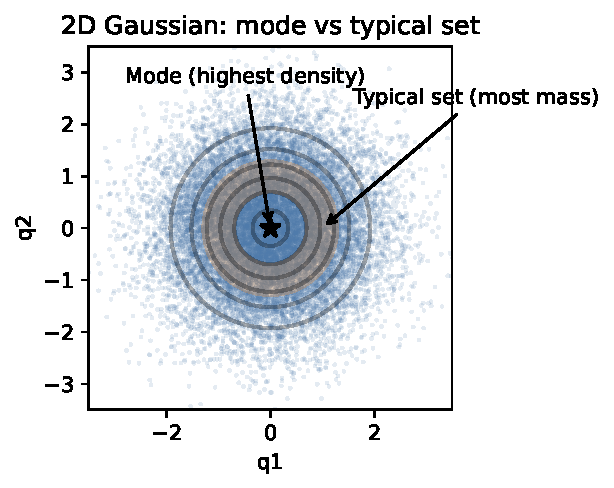
\includegraphics[width=0.46\textwidth]{mode_vs_typical_set.pdf} 
	\end{figure}
\end{frame}

\begin{frame}{Physical Interpretation}
	\textbf{Neal, 2011}

	\textit{
		In two dimensions, we can visualize the dynamics as that of a frictionless puck that
		slides over a surface of varying height. The state of this system consists of the
		position of the puck, given by a $2D$ vector $q$, and the momentum of the puck
		(its mass times its velocity), given by a $2D$ vector $p$.}

	\vspace{0.5cm}
	\textit{
		On a level part of the surface, the puck moves at a constant velocity.
		If it encounters a rising slope, the puck's momentum allows it to continue, with its
		kinetic energy $K(p)$ decreasing and its potential energy $U(q)$ increasing, until the kinetic energy
		is zero, at which point it will slide back down (with kinetic energy increasing and
		potential energy decreasing)}
\end{frame}

\begin{frame}{Hamiltonian Equation}
	Our target distribution is defined in terms of a potential energy function $U(q)$,
	which encodes the negative log probability of the target distribution $\pi(q)$ that we wish to sample from.

	We extend the state space by introducing auxiliary variables and sample from $\pi$ with density:
	
	\begin{equation*}
		\pi(q, p) \propto \exp(-H(q, p)) = \exp(-U(q)) \exp(-K(p))	
	\end{equation*}

	where $H(q, p)$ is the Hamiltonian function, representing the total energy of the system,
	given by the sum of kinetic and potential energy:

	\begin{equation*}
		H(q, p) = U(q) + K(p) = U(q) + \frac{1}{2} p^T M^{-1} p
	\end{equation*}
	Note that marginalizing $p$ recovers the target distribution $\pi(q)$.
\end{frame}

\begin{frame}{Hamiltonian Dynamics}
	How to propose new states $(q, p)$? We simulate Hamiltonian dynamics to generate proposals that
	preserve the Hamiltonian (total energy) of the system. Exact Hamiltonian dynamics preserve both energy and volume; in discrete time, leapfrog approximately preserves energy but exactly preserves volume.
	
	\vspace{0.4cm}
	The dynamics of the system can be described by these equations,
	\begin{equation*}
		\frac{dq}{dt} = \frac{\partial H}{\partial p} \quad \text{and} \quad
		\frac{dp}{dt} = -\frac{\partial H}{\partial q}
	\end{equation*}
	which govern
	the time evolution of the position and momentum variables. How do we simulate these dynamics 
	in discrete time? We use the Leapfrog integrator.
\end{frame}

\begin{frame}{Leapfrog Integrator}
	To numerically simulate Hamiltonian dynamics, we use the leapfrog integrator, which is a
	symplectic method that preserves the volume in phase space and is time-reversible
	up to a momentum flip; that’s why we often negate p at the end of the trajectory.
	\begin{align*}
		p\left(t + \frac{\varepsilon}{2}\right) & = p(t) - \frac{\varepsilon}{2} \nabla U(q(t))                                                  \\
		q(t + \varepsilon)                      & = q(t) + \varepsilon M^{-1} p\left(t + \frac{\varepsilon}{2}\right)                            \\
		p(t + \varepsilon)                      & = p\left(t + \frac{\varepsilon}{2}\right) - \frac{\varepsilon}{2} \nabla U(q(t + \varepsilon))
	\end{align*}
	where $\varepsilon$ is the step size.

	\vspace{0.4cm}
	Being symplectic means that this transformation preserves volume in phase space and
	that the Jacobian determinant of the transformation is equal to one and hence the Metropolis
	Acceptance ratio needs no volume correction factor.
\end{frame}

\begin{frame}
	\begin{block}{Vanilla HMC Algorithm}
		Requires: Leapfrog integrator $\varphi$, step-size $\varepsilon$, number of steps $L$, current position $q$
		and positive definite matrix $M$.

		\begin{enumerate}
			\item \textbf{Energy lift}: given $q$, draw $p \sim N(0, M)$  - (random) \\
			      This "lifts" our position into phase space by adding kinetic energy

			\item \textbf{Hamilton flow}: propose $q^*, p^* = \varphi_{\varepsilon}^L(q, p)$ - (deterministic)\\
			      Simulate dynamics for $L$ steps using leapfrog integrator. Follow energy-conserving  \\
			      trajectory through phase space. 

			\item \textbf{Metropolis acceptance step} - (random) \\
			      accept $q^*$ with probability
			      $\min\Big\{1, \exp(H(q, p) - H(q^*, p^*))\Big\}$ \\
			      Corrects for numerical errors in integration. No Jacobian term; leapfrog is volume-preserving
		\end{enumerate}
	\end{block}
	Note $H(q^*, -p^*) = H(q^*, p^*)$ because the $K$ is even in $p$, so the minus is redundant.
\end{frame}

\begin{frame}{Choosing parameters in HMC}
	\textbf{Another story...}
	\vspace{0.5cm}

	\textbf{Step-size $\varepsilon$}: optimal scaling

	\begin{itemize}
		\item Dimension dependence of stepsize:
		      \begin{itemize}
			      \item RWM: $\bigO(d^{-1})$
			      \item MALA: $\bigO(d^{-1/3})$
			      \item HMC: $\bigO(d^{-1/4})$
		      \end{itemize}
		\item Optimal acceptance rates:
		      \begin{itemize}
			      \item RWM: 0.234
			      \item MALA: 0.574
			      \item HMC: 0.651
		      \end{itemize}
	\end{itemize}
	\vspace{0.5cm}
	\textbf{Choose $L$ adaptively}: NUTS sampler
\end{frame}
